\begin{frame}{Xử lý lệch thứ tự tạo và thu hồi liên kết chia sẻ}
\begin{figure}[H]
\centering
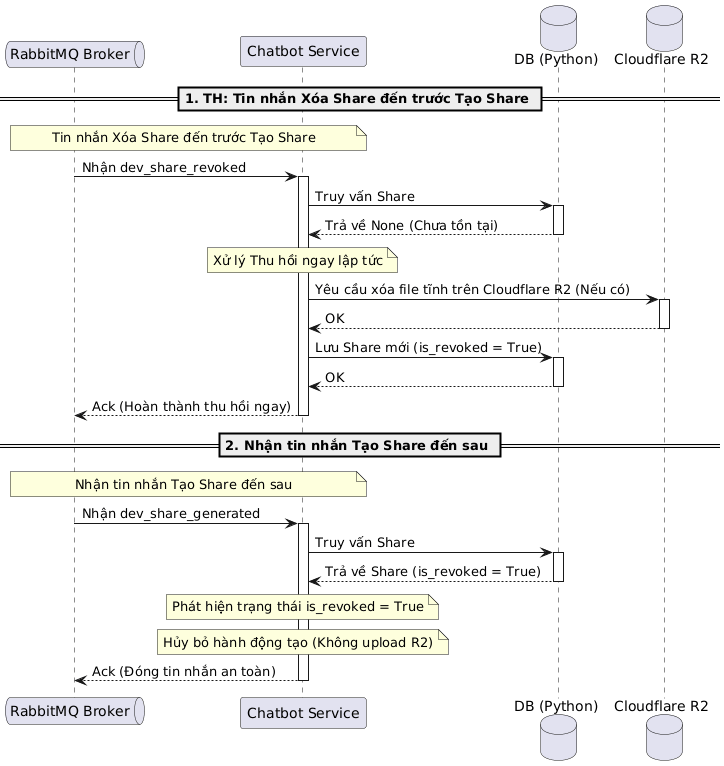
\includegraphics[height=0.7\textheight,width=0.9\textwidth,keepaspectratio]{pictures/share-out-of-order.png}
\caption{Sơ đồ xử lý lệch thứ tự tạo và thu hồi chia sẻ}
\end{figure}

\note{
Trong hệ thống phân tán, do các tác vụ xử lý tệp tin và upload lên Cloudflare R2 được thực hiện bất đồng bộ qua RabbitMQ, có thể xảy ra hiện tượng lệch thứ tự tin nhắn (out-of-order).
Ví dụ, yêu cầu thu hồi chia sẻ đến trước khi quá trình upload hoàn tất. Để xử lý, hệ thống sử dụng cơ chế kiểm tra trạng thái trong Database. Khi nhận sự kiện thu hồi, hệ thống ghi nhận trạng thái đã thu hồi vào DB, nhờ đó khi tác vụ upload hoàn tất sau đó, hệ thống sẽ tự động xóa file trên R2 ngay lập tức.
}
\end{frame}
